\begin{flushleft}
Iniciamos una nueva conexión con el SQL DEVELOPER, aquí colocaremos, nombre de la conexión, el usuario sys, contraseña: Oracle, Tipo de conexión Básico, Rol: SYSDBA, Nombre del host: localhost, puerto 1521, SID: orcl\\
\begin{center}
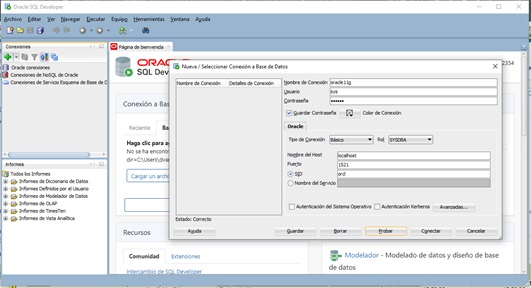
\includegraphics{images/image-18}\\
\end{center}
Una vez conectados creamos el usuario DBA1 y le otorgamos permisos con el comando GRANT\\
\begin{center}
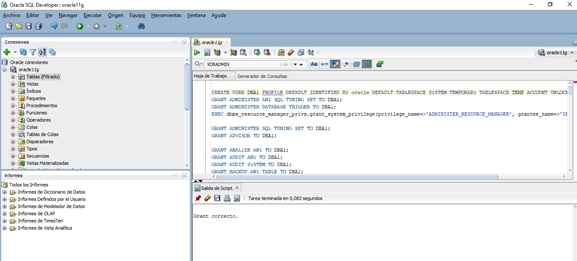
\includegraphics{images/image-19}\\
\end{center}
En este paso regresamos a la URL del ENTERPRISE MANAGE DATABASE CONTROL y nos dirigimos a link Configurar situado en la parte derecha superior de la ventana\\
\begin{center}
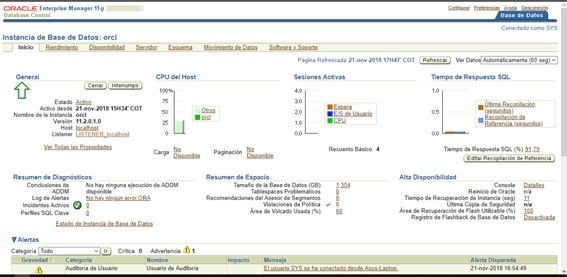
\includegraphics{images/image-20}\\
\end{center}
Después de hacer Clic nos mostrara la página de configuración, en donde damos clic en el link Administradores del menú situado al lado izquierdo de la ventana\\
\begin{center}
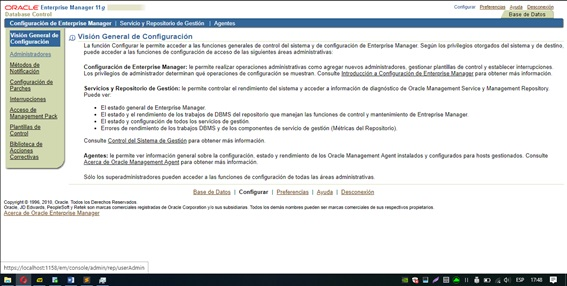
\includegraphics{images/image-21}\\
\end{center}
Después nos cargara esta página donde presionamos en el botón crear\\
\begin{center}
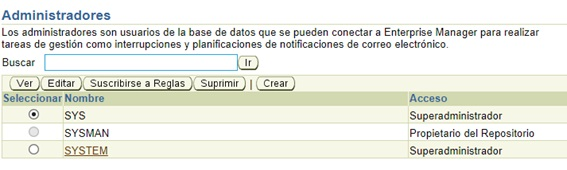
\includegraphics{images/image-22}\\
\end{center}
En esta página seleccionaremos el usuario previamente creado, asignaremos una dirección de correo electrónico y cambiamos el privilegio de administrador a SUPERADMINISTRADOR\\
\begin{center}
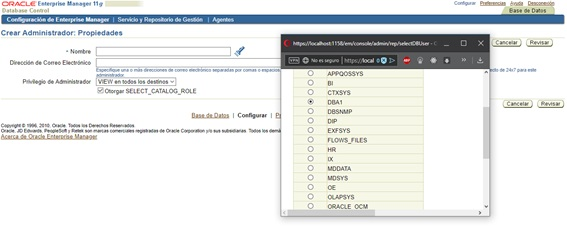
\includegraphics{images/image-23}\\
\end{center}
En esta página seleccionaremos al usuario DBA1 y luego presionamos en el botón seleccionar\\
\begin{center}
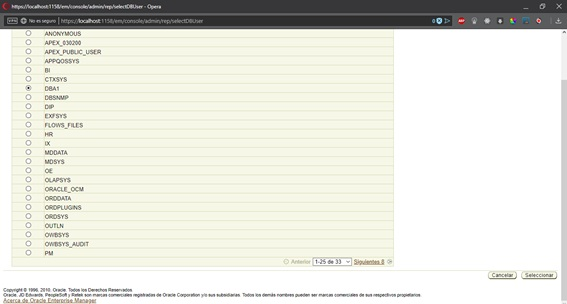
\includegraphics{images/image-24}\\
\end{center}
Una vez llenado el formulario para crear al USUARIO DBA1, presionamos en el botón revisar\\
\begin{center}
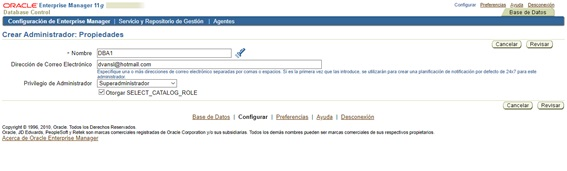
\includegraphics{images/image-25}\\
\end{center}
Luego nos saldrá otra página para confirmar la creación, para ello presionamos en el botón Terminar\\
\begin{center}
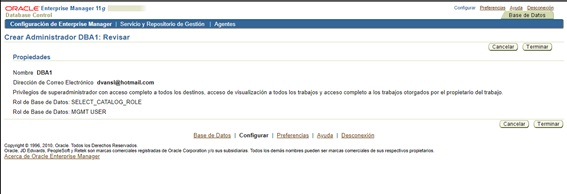
\includegraphics{images/image-26}\\
\end{center}
Luego verificamos en la página de Administrador, en donde debe figurar nuestro usuario debidamente creado\\
\begin{center}
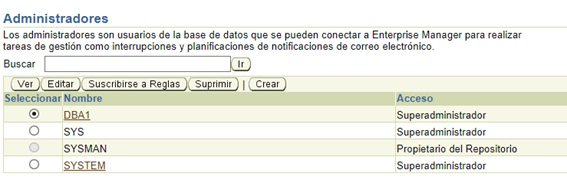
\includegraphics{images/image-27}\\
\end{center}
En este paso crearemos un tablespace para nuestro proyecto, para ellos nos dirigimos a la pestaña Servidor y luego al link Tablespaces\\
\begin{center}
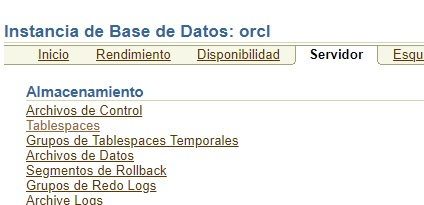
\includegraphics{images/image-28}\\
\end{center}
Luego nos mostrara la página para crear un tablespace\\
\begin{center}
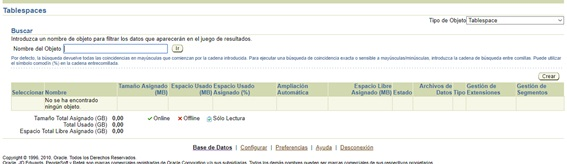
\includegraphics{images/image-29}\\
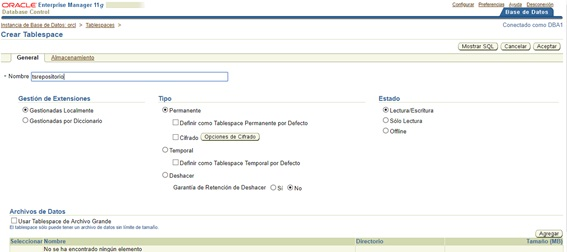
\includegraphics{images/image-30}\\
\end{center}
En esta ventana crearemos una tabla de espacio para nuestra base de datos, para ellos llenaremos todos los campos necesarios del formulario y luego presionamos en el botón continuar\\
\begin{center}
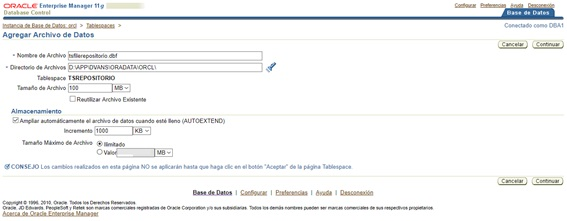
\includegraphics{images/image-31}\\
\end{center}
Luego en esta ventana colocaremos el nombre de la tabla de espacio y presionaremos en el botón aceptar\\
\begin{center}
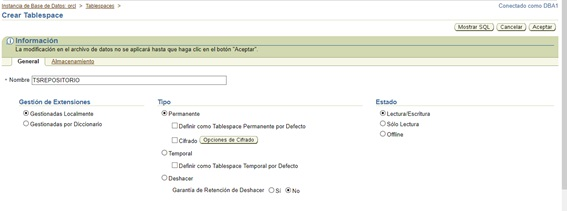
\includegraphics{images/image-32}\\
\end{center}
Finalmente en esta parte verificamos que nuestra tabla de espacio este en la lista de tabla de espacio\\
\begin{center}
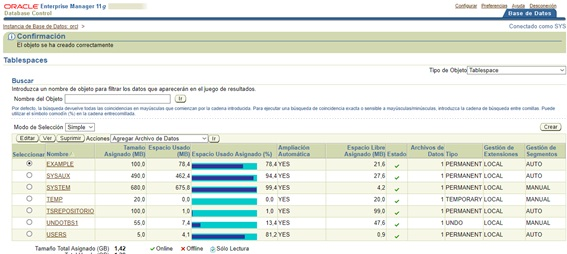
\includegraphics{images/image-33}\\
\end{center}
Finalmente crear las tablas de nuestra base de datos y las relacionaremos con el esquema DBA1\\
\begin{center}
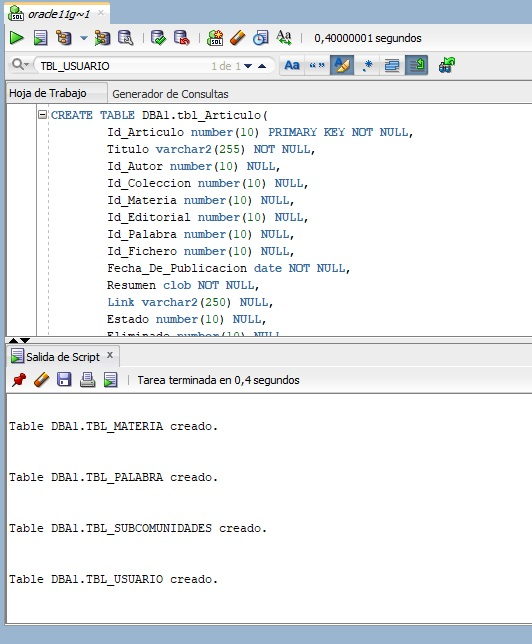
\includegraphics{images/image-34}\\
\end{center}
\end{flushleft}